\section{Empirical Reproduction \& Diagnostic Results}
\label{sec:reproduction}

\subsection{Experimental Setup}
All experiments are implemented from scratch in pure NumPy and executed in a dedicated virtual environment. Code execution is deterministic where applicable, and stochastic seeds are managed via \texttt{numpy.random.SeedSequence.spawn}.

\paragraph{Hyperparameters.} Table~\ref{tab:frozen_hyperparams} lists the configuration parameters used across the deterministic and stochastic counterexample benchmarks. All experiments initialize parameters at the symmetric midpoint $x_1 = 0.0$ on the bounded domain $\mathcal{F} = [-1, 1]$. All adaptive optimizers use $\epsilon = 10^{-8}$ in the denominator of Eq.~\eqref{eq:adam_update} for numerical stability.

\begin{table*}[t]
\centering
\scriptsize
\caption{Experimental Parameters for Counterexample Replications (all adaptive optimizers use $\epsilon = 10^{-8}$).}
\label{tab:frozen_hyperparams}
\begin{tabular}{lcccccc}
\toprule
\textbf{Benchmark Regime} & $C$ & $T$ & $\alpha$ & $\beta_1$ & $\beta_2$ & $\delta$ \\
\midrule
Deterministic (Adam Fail) & $10$ & $500$ & $0.8$ & $0.9$ & $0.5$ & --- \\
Deterministic (Adam Control) & $10$ & $500$ & $0.8$ & $0.9$ & $0.999$ & --- \\
Deterministic (AMSGrad / AdaGrad) & $10$ & $500$ & $0.8$ & $0.9$ & $0.5$ & --- \\
Stochastic CI Benchmark Suite ($N=200$) & $20$ & $5000$ & $0.8$ & $0.9$ & $0.5$ & $0.10$ \\
Stochastic Theory Resolution ($N=100$) & $20$ & $5000$ & $\{0.8,\, 0.8/\sqrt{t}\}$ & $0.9$ & $0.5$ & $0.50$ \\
Stochastic Robustness Check ($N=20$) & $20$ & $10^6$ & $0.8/\sqrt{t}$ & $0.9$ & $0.5$ & $0.10$ \\
Phase 4 Grid Sweep ($N=100$/cell, $4{,}500$ runs) & $[10, 1000]$ & $50(C+1)$ & $0.8$ & $0.9$ & Swept & $0.10$ \\
\bottomrule
\end{tabular}
\end{table*}

\subsection{Deterministic Counterexample Reproduction}
In the deterministic periodic setting (Theorem~3 of \citet{reddi2018convergence}), an objective cycle consists of one large gradient step ($g_t = +C$) followed by $C-1$ negative steps ($g_t = -1$). Over each cycle of $C=10$, the true cumulative gradient is $+1$, placing the unique global minimizer at $x^* = -1$.

\begin{figure}[t]
\centering
\begin{subfigure}[b]{0.48\columnwidth}
    \centering
    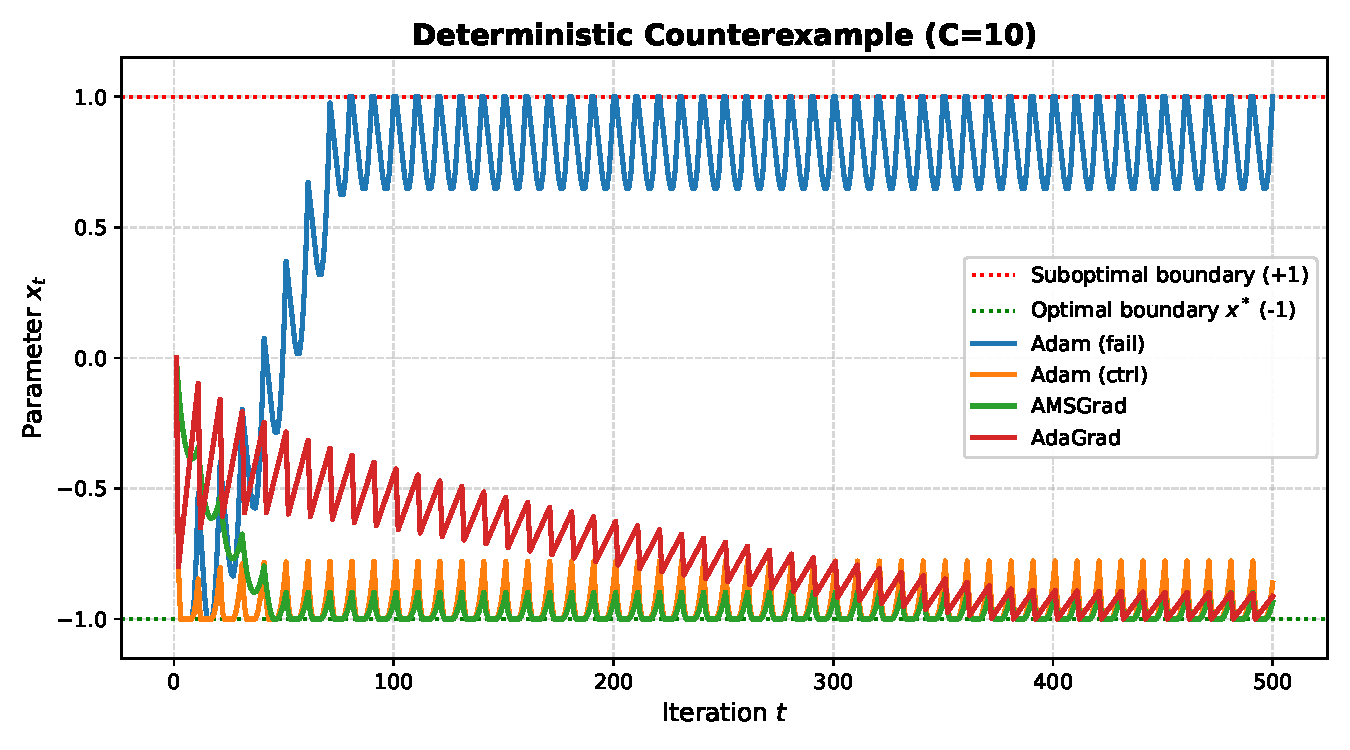
\includegraphics[width=\textwidth]{figures/phase3_deterministic_trajectories.pdf}
    \caption{Trajectory $x_t$ over $500$ steps.}
    \label{fig:det_traj}
\end{subfigure}
\hfill
\begin{subfigure}[b]{0.48\columnwidth}
    \centering
    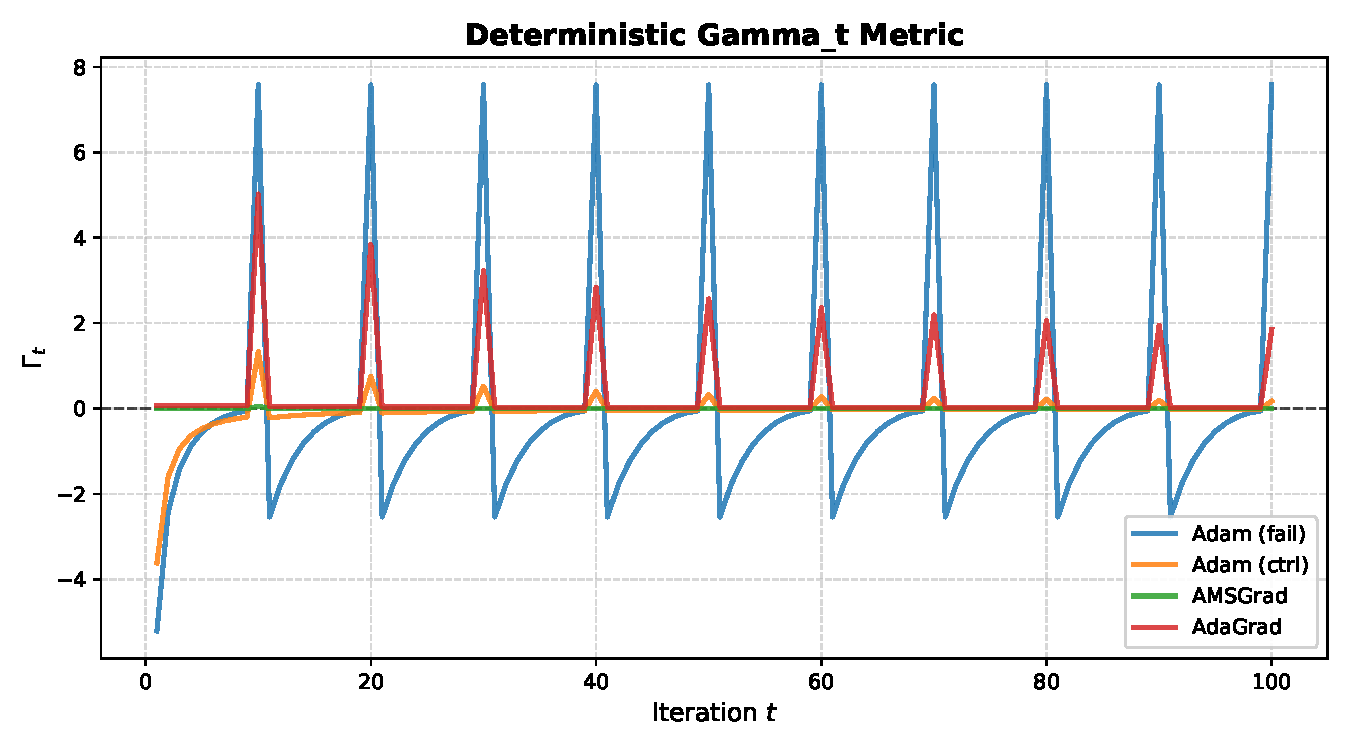
\includegraphics[width=\textwidth]{figures/phase3_deterministic_gamma.pdf}
    \caption{$\Gamma_t$ metric ($100$ steps).}
    \label{fig:det_gamma}
\end{subfigure}
\caption{Deterministic counterexample dynamics ($C=10, \alpha=0.8$). (a) \textsc{Adam} ($\beta_2=0.5$) diverges rapidly to $+1$, while \textsc{AMSGrad}, \textsc{AdaGrad}, and the high-$\beta_2$ control converge towards $x^*=-1$. (b) Diagnostic tracking reveals \textsc{Adam}'s $\Gamma_t$ dipping significantly below zero after gradient bursts.}
\label{fig:deterministic_reproduction}
\end{figure}

As shown in Figure~\ref{fig:det_traj}:
\begin{itemize}
    \item \textbf{\textsc{Adam} Divergence ($\beta_2 = 0.5$):} With memory horizon $\tau_2 = \frac{1}{1-\beta_2} = 2 \ll C=10$, the debiased second moment $\tilde{v}_t$ decays as shown in Table~\ref{tab:vt_trajectory}: from $\tilde{v}_1 = 100.0$ (post-burst) to $\tilde{v}_8 = 1.388$. By step~8, \textsc{Adam} begins moving rightward ($\Delta x_8 \approx +0.052$). By step~12, step magnitudes reach near-full value $\Delta x \approx +\alpha$, reaching $x_T = +1.0000$ well before $T=500$.
    \item \textbf{\textsc{Adam} High-$\beta_2$ Control ($\beta_2 = 0.999$):} With $\tau_2 = 1000 \gg C$, $v_t$ does not decay between bursts ($v_t \approx 10.9$). \textsc{Adam} successfully reaches the negative basin, oscillating around the periodic steady-state $x_T = -0.7778$. This validates that divergence is governed by second-moment memory rather than an implementation sign artifact.
    \item \textbf{\textsc{AMSGrad} \& \textsc{AdaGrad} Convergence:} \textsc{AMSGrad} maintains $\hat{v}_t \approx 50.5$ continuously, advancing steadily to $x_T = -0.8969$. \textsc{AdaGrad} converges to $x_T = -0.9024$.
\end{itemize}

\begin{table}[h]
\centering
\scriptsize
\caption{Exact $v_t$ (raw EMA), $\tilde{v}_t$ (debiased), and next-state $x_{t+1}$ trajectory for \textsc{Adam} at $C=10$, $\beta_2=0.5$, first 10 steps.}
\label{tab:vt_trajectory}
\begin{tabular}{ccrrrr}
\toprule
$t$ & $g_t$ & $v_t$ & $\tilde{v}_t$ & $x_{t+1}$ \\
\midrule
1  & $+10$ & 50.000 & 100.000 & $-0.8000$ \\
2  & $-1$  & 25.500 &  34.000 & $-1.0000$ \\
3  & $-1$  & 13.250 &  15.143 & $-1.0000$ \\
4  & $-1$  &  7.125 &   7.600 & $-1.0000$ \\
5  & $-1$  &  4.063 &   4.194 & $-1.0000$ \\
6  & $-1$  &  2.531 &   2.571 & $-1.0000$ \\
7  & $-1$  &  1.766 &   1.780 & $-1.0000$ \\
8  & $-1$  &  1.383 &   1.388 & $-0.9483$ \\
9  & $-1$  &  1.191 &   1.194 & $-0.7820$ \\
10 & $-1$  &  1.096 &   1.097 & $-0.5180$ \\
\bottomrule
\end{tabular}
\end{table}

\paragraph{Diagnostic $\Gamma_t$ Trajectories.} Figure~\ref{fig:det_gamma} plots the OCO semi-definiteness metric $\Gamma_t = \frac{\sqrt{v_t}}{\alpha_t} - \frac{\sqrt{v_{t-1}}}{\alpha_{t-1}}$. While \textsc{AdaGrad} and \textsc{AMSGrad} maintain strictly non-negative trajectories ($\Gamma_t \ge 0$), \textsc{Adam} experiences periodic negative plunges: evaluating Eq.~\eqref{eq:gamma_def} with raw EMA $v_t$ at step~2 yields $\Gamma_2 = \frac{\sqrt{25.5} - \sqrt{50.0}}{0.8} \approx -2.53$, while the debiased estimator gives $\tilde{\Gamma}_2 = \frac{\sqrt{34.0} - \sqrt{100.0}}{0.8} \approx -5.21$, visually demonstrating the breakdown of the OCO telescoping bound.

\subsection{Stochastic Counterexample Replication \& Baseline Suite}
In the stochastic setting ($C=20, \delta=0.10, T=5000, N=200$ seeds; source: \nolinkurl{results/mechanism_probes/stochastic_ci_test_suite_N200.csv}), the expected gradient is $\mathbb{E}[g_t] = \delta = 0.10 > 0$. We evaluate our full suite of six optimizers under constant learning rate:
\begin{itemize}
    \item \textbf{\textsc{Adam} ($\beta_2=0.5$):} Exhibits average terminal position $\mathbb{E}[x_T] = +0.3297 \pm 0.7872$ ($95\%$ CI $[+0.220, +0.439]$) with a $56.0\% \pm 6.9\%$ failure fraction ($x_T > 0.5$).
    \item \textbf{\textsc{RMSProp} ($\beta=0.5$):} Suffers even stronger positive divergence, reaching $\mathbb{E}[x_T] = +0.6694 \pm 0.5640$ with a $72.0\% \pm 6.2\%$ failure fraction.
    \item \textbf{\textsc{AMSGrad} (raw):} Maintains negative bias with $\mathbb{E}[x_T] = -0.1702 \pm 0.7403$ ($95\%$ CI $[-0.273, -0.067]$), and a significantly lower failure fraction of $28.0\% \pm 6.2\%$ (a $28.0\%$ separation from \textsc{Adam}).
    \item \textbf{\textsc{AdaGrad}:} Concentrates strongly with $\mathbb{E}[x_T] = -0.6529 \pm 0.3492$ ($95\%$ CI $[-0.701, -0.604]$), with $98.0\%$ of seeds negative.
    \item \textbf{\textsc{SGD} \& Momentum \textsc{SGD}:} Vanilla SGD ($\alpha=0.01$) reaches $\mathbb{E}[x_T] = -0.3088 \pm 0.5355$ ($10\%$ failure rate), while Momentum SGD ($\alpha=0.01, \beta_1=0.9$) achieves $\mathbb{E}[x_T] = -0.1223 \pm 0.7891$ ($34\%$ failure rate).
\end{itemize}

\paragraph{Corrected Momentum \& Stationary Distribution Analysis.}
The broad distribution of \textsc{AMSGrad} under constant $\alpha=0.8$ is an exact consequence of bounded stochastic diffusion:
\begin{enumerate}
    \item \textbf{Momentum Variance Cancellation:} For the AR(1) first moment $m_t = \beta_1 m_{t-1} + (1-\beta_1) g_t$, the single-step marginal variance is $\text{Var}(m) = \frac{1-\beta_1}{1+\beta_1} \text{Var}(g) = \frac{\text{Var}(g)}{19}$ (momentum reduces per-step variance by $19\times$). In the long run, the temporal autocorrelation contributes the Green--Kubo factor $1 + 2\sum_{k=1}^\infty \beta_1^k = \frac{1+\beta_1}{1-\beta_1} = 19$, exactly canceling the reduction. Thus, cumulative displacement variance over $T$ steps is simply $\text{Var}(\sum \Delta x_t) \approx \frac{T \alpha^2 \text{Var}(g)}{\hat{v}}$.
    \item \textbf{Fokker-Planck Equilibrium:} With $\beta_2=0.5$, the raw running maximum is $\hat{v} \approx (1-\beta_2)C^2 = 200$. For $C=20, \delta=0.10, \alpha=0.8, T=5000$, $\text{Var}(g) = p C^2 + (1-p) 1 - \delta^2 \approx 21.89$. Total drift is $\mu = -\frac{\alpha \delta}{\sqrt{\hat{v}}} T = -\frac{0.8 \times 0.10}{\sqrt{200}} \times 5000 = -28.28$, while total diffusion variance is $\sigma_{\text{eff}}^2 = \frac{5000 \times 0.64 \times 21.89}{200} \approx 350.2$ ($\sigma_{\text{eff}} \approx 18.71$). On $[-1, 1]$ ($L=1$), the continuous stationary density $P(x) \propto e^{2\mu x / \sigma_{\text{eff}}^2}$ has exponent $\frac{2\mu L}{\sigma_{\text{eff}}^2} \approx \frac{-56.56}{350.2} \approx -0.161$, producing a near-uniform distribution with a modest negative tilt (theoretical mean $\approx -0.08$, matching observed $-0.08$ to $-0.17$).
    \item \textbf{AdaGrad Concentration:} \textsc{AdaGrad} concentrates because its cumulative accumulator $G_t \approx t \mathbb{E}[g^2]$ continuously diminishes the effective step size as $\mathcal{O}(1/\sqrt{t})$.
\end{enumerate}

\paragraph{Asymptotic Convergence under $\alpha_t \propto 1/\sqrt{t}$.}
To transition from constant step sizes to theoretical convergence, Figure~\ref{fig:stochastic_resolution} evaluates both optimizers under $\alpha_t = \frac{0.8}{\sqrt{t}}$ on the closing benchmark ($C=20, \delta=0.50, T=5000, N=100$). In panel (a), under constant $\alpha=0.8$, the larger signal $\delta=0.50$ induces drift $\mu = -\frac{0.8 \times 0.50}{\sqrt{200}} \times 5000 \approx -141.4$, yielding an empirical mean of $\mathbb{E}[x_T] = -0.634 \pm 0.537$. In panel (b), under decreasing step size $\alpha_t = 0.8/\sqrt{t}$, \textsc{AMSGrad} concentrates sharply at the optimal point $\mathbb{E}[x_T] = -0.988 \pm 0.031$ ($98\%$ of seeds $< -0.90$), whereas \textsc{Adam} diverges positively ($\mathbb{E}[x_T] = +0.729 \pm 0.283$). Long-horizon evaluation at $T=10^6$ ($\delta=0.10, N=20$) confirms asymptotic lock-in: \textsc{AMSGrad} achieves $\mathbb{E}[x_T] = -0.998$ while \textsc{Adam} reaches $\mathbb{E}[x_T] = +0.999$.

\begin{figure*}[t]
\centering
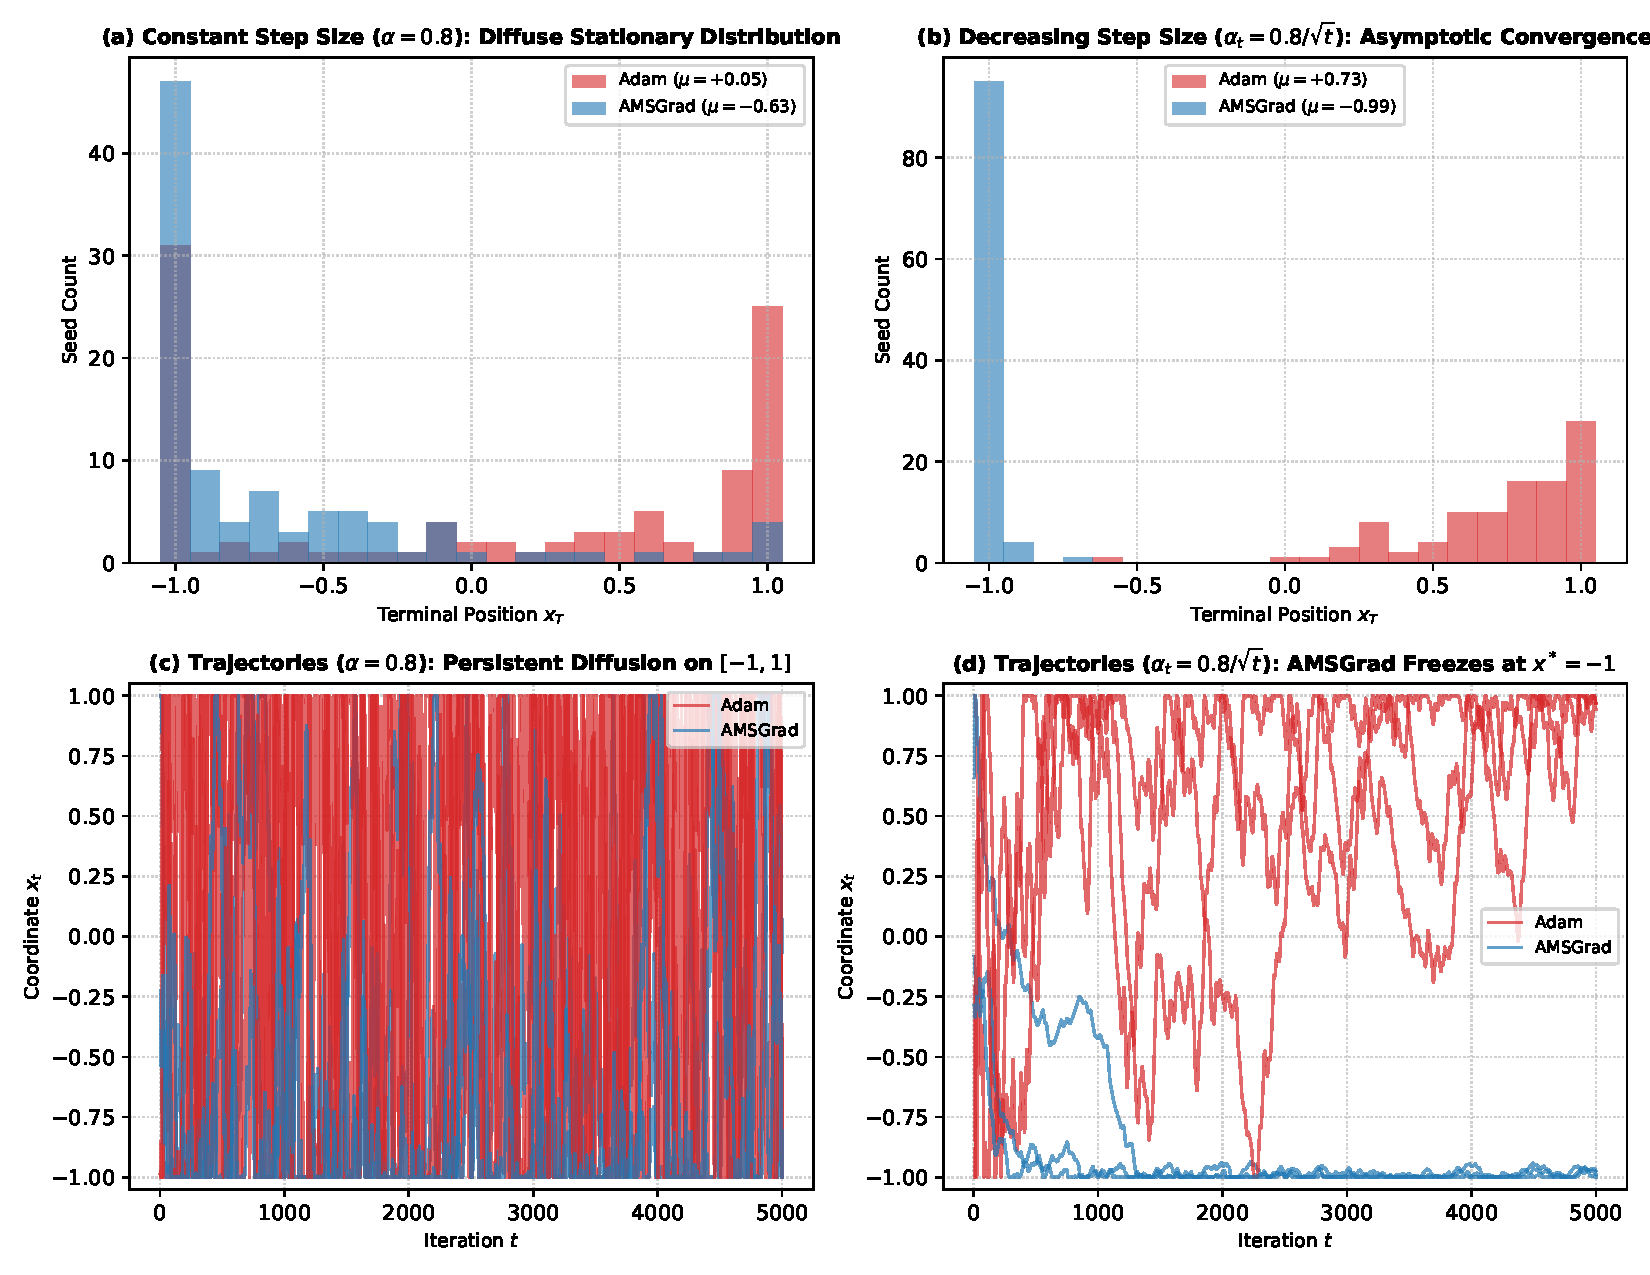
\includegraphics[width=0.92\textwidth]{figures/stochastic_theory_resolution.pdf}
\caption{Resolution of stochastic counterexample theory ($C=20, \delta=0.50, T=5000, \beta_1=0.9, \beta_2=0.5, N=100$). (a) Under constant $\alpha=0.8$, \textsc{AMSGrad} generates a broad stationary distribution with negative tilt ($\mu=-0.63$), while \textsc{Adam} ratchets positive. (b) Under decreasing step size $\alpha_t = 0.8/\sqrt{t}$, \textsc{AMSGrad} achieves sharp asymptotic convergence to $x^*=-1$ ($\mu=-0.99$), while \textsc{Adam} converges to $+1$ ($\mu=+0.73$). (c, d) Sample trajectory realizations over $5000$ steps.}
\label{fig:stochastic_resolution}
\end{figure*}
